\documentclass[12pt]{article}

\usepackage[margin=1in]{geometry}	% margin settings
\usepackage{amsfonts, amsmath, amssymb}	% symbols and environments for math
%\usepackage[none]{hyphenat}	% prevent hyphenation of text
\usepackage{graphicx}
\usepackage{import}
\usepackage{float}
\usepackage{hyperref}	% provide ability to have pdf links
\usepackage{xcolor}

\setlength{\parindent}{0em}	% indentation of new paragraph
\setlength{\parskip}{0.5em}	% spacing between paragraphs
\renewcommand{\baselinestretch}{1}	% line-spacing

%opening
\title{Latex Technical Guide By Me}
\author{H.W. Jordaan}

\begin{document}

\maketitle

\section*{What does this guide contain?}
\LaTeX~is a powerful tool to generate beautifully styled documents.
It can be very intimidating and confusing when constructing your first document.
The first time you apply it, it will feel as if the basic things will take forever.
A common concern is: ``How will I ever remember all these commands?''
This is normal, and I can tell you that there is light in that very dark tunnel.

The aim of this guide is to not cover the basics - that is what the internet and YouTube is for.
Rather, this document will give you hints how to do certain common parts, and also share best practices, when you are constructing a formal academic document such as a research report, research paper or thesis.

The majority of this document should not be read from the start to the end, but should rather serve be referred to while writing and want advice in how to do a certain thing.
Each section of this guide will try and cover a single question or component.

\section*{When should I use \LaTeX?}
Some converts will say: ``It the best thing ever.  For everything of course.''
Some others which are intimidated or have not have a good start relationship will respond: ``It is too complex!  Just use Word.''

Well the fact is that \LaTeX~is not commonly used in industry and is mainly reserved for the small community of researchers and academics of the world.
I believe \LaTeX~shines when your document fulfils in the following characteristics:
\begin{enumerate}
	\item Will be very large - 100 plus pages
	\item Will have a large number of mathematical equations
	\item Will contain a large number of references and citations
\end{enumerate}

If your are new to \LaTeX~or are looking for information for doing something simple please refer to the YouTube videos within the following channels:
\begin{itemize}
	\item \url{https://www.youtube.com/user/mrskrummel}
	\item \url{https://www.youtube.com/playlist?list=PLNnwglGGYoTtW7o4PHFOSWGevcdFa3v3D}
	\item \url{https://www.youtube.com/user/ShareLaTeX}
	\item \url{https://www.youtube.com/channel/UC3gO3p5rBvmTpPHp0xHMluQ}
\end{itemize}

\section*{Which editor should I use?}
This is simple.
It does not matter.
There are many IDEs for writing \LaTeX: TexStudio (suggested), TexLive, TeXnicCenter, Kile or just a standard text editor.
These tools have variable difficulty to setup, but when installed everything runs on your local machine and compiling is as fast as your system can do it.

Another option is to make use of an online platform such as Overleaf (suggested) or ShareLatex.
These tools are great if you are new to \LaTeX, want to share and work together on a document with someone and want a cloud-based solution.
The drawbacks are that this method is less useful for when document gets larger (compile time increases), you always need internet connectivity and it is more awkward to upload pictures.

Final opinion:  If this is your first time using \LaTeX~or want to write something small such as an article with or without collaborators use an online platform.
Larger documents such as a thesis (Masters or PhD) you should start looking at a local installation.

\section*{Is there a right way to write the source?}
Well simply if it compiles then it is probably okay.
There are a number of suggestions for when the document get really big or when you are collaborating with other people.
Here follows a list of the highlight real:
\begin{itemize}
	\item 
\end{itemize}

\section*{How to handle figures}
This is probably the thing I have spent the most of my \LaTeX~writing time, and have tried a number of different methods.
Yes, you can simply just generate a plot in Matlab, export a .png and import it.
If you want to exploit the power of \LaTeX~there is a little bit more to it to really get that next level picture or graph.
If you want to do it right you will need to be prepared to put in the time in, but the result will be beautiful and the readers will fall to the floor when they turn that page.
The basic concerns when creating a figure is:
\begin{enumerate}
	\item Resolution - in this regards vector based is always better and provide a balance between quality of rendering and size of image.
	\item Size - figures with font normally scale with the rest of the figure thus relative size of fonts in figure and rest of text changes
	\item Repeatability - consistently create multiple graphs and diagrams which have the same size and style
	\item Effort - process must not be over time consuming and too clicky-clicky (queue mouse button sound)
\end{enumerate}
In most documents you will be faced with three possible figures which will be discussed separately:
\begin{enumerate}
	\item Pictures
	\item Diagrams
	\item Graphs
\end{enumerate}

\subsection*{How to handle pictures}
\url{https://youtu.be/GaI1RdFNtA8}
\begin{itemize}
	\item Vector-based drawing in Inkscape
	\item Inkscape is cross-platform
	\item Copy in image from Google and trace over with line in Inkscape to get good realistic pictures
	\item Labels and text use Latex notation
	\item Save image as Pdf but with the Text output options \textit{Omit text in PDF and create LaTeX file}
	\item Include the generate .tex file in the document source. 
\end{itemize}
%\begin{figure}[!h]
%	\centering
%	\import{figures/}{test_picture.pdf_tex}
%	\caption{This is an example of a good vector picture.}
%	\label{fig:testpicture}
%\end{figure}

\subsection*{How to handle diagrams}
\begin{itemize}
	\item Use Inkscape to create diagram, similar to process described to create a picture
	\item Use Tikz to generate your block diagram
\end{itemize}

\begin{figure}[!h]
	\centering
	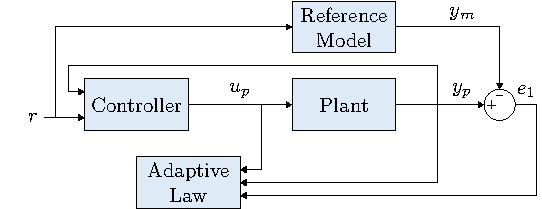
\includegraphics{figures/test_diagram}
	\caption{This is an example of a good diagram.}
	\label{fig:testdiagram}
\end{figure}

\subsection*{How to handle graphs}
\url{https://youtu.be/JgXukrKZ9X8?list=PL5fGdFBgOr6N9w2YLk-T623YQAcnqtcYt}
\begin{itemize}
	\item Generate the figure in Tikz
	\item Have the graph data in .csv files
\end{itemize}

\begin{figure}[!h]
	\centering
	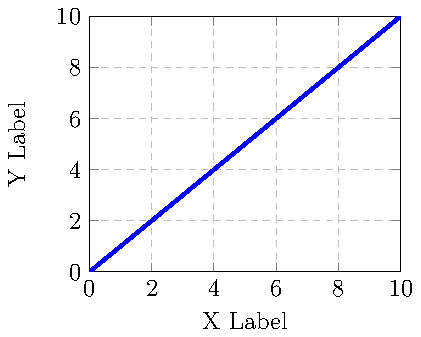
\includegraphics{figures/test_graph}
	\caption{This is an example of a good graph.}
	\label{fig:testgraph}
\end{figure}


\subsection*{Fixing the compile time of these figures}

\end{document}